% Options for packages loaded elsewhere
\PassOptionsToPackage{unicode}{hyperref}
\PassOptionsToPackage{hyphens}{url}
\PassOptionsToPackage{dvipsnames,svgnames,x11names}{xcolor}
%
\documentclass[
  11pt,
]{article}
\author{}
\date{\vspace{-2.5em}}

\usepackage{amsmath,amssymb}
\usepackage{lmodern}
\usepackage{iftex}
\ifPDFTeX
  \usepackage[T1]{fontenc}
  \usepackage[utf8]{inputenc}
  \usepackage{textcomp} % provide euro and other symbols
\else % if luatex or xetex
  \usepackage{unicode-math}
  \defaultfontfeatures{Scale=MatchLowercase}
  \defaultfontfeatures[\rmfamily]{Ligatures=TeX,Scale=1}
  \setmainfont[]{Palatino}
\fi
% Use upquote if available, for straight quotes in verbatim environments
\IfFileExists{upquote.sty}{\usepackage{upquote}}{}
\IfFileExists{microtype.sty}{% use microtype if available
  \usepackage[]{microtype}
  \UseMicrotypeSet[protrusion]{basicmath} % disable protrusion for tt fonts
}{}
\makeatletter
\@ifundefined{KOMAClassName}{% if non-KOMA class
  \IfFileExists{parskip.sty}{%
    \usepackage{parskip}
  }{% else
    \setlength{\parindent}{0pt}
    \setlength{\parskip}{6pt plus 2pt minus 1pt}}
}{% if KOMA class
  \KOMAoptions{parskip=half}}
\makeatother
\usepackage{xcolor}
\IfFileExists{xurl.sty}{\usepackage{xurl}}{} % add URL line breaks if available
\IfFileExists{bookmark.sty}{\usepackage{bookmark}}{\usepackage{hyperref}}
\hypersetup{
  colorlinks=true,
  linkcolor={teal},
  filecolor={Maroon},
  citecolor={teal},
  urlcolor={teal},
  pdfcreator={LaTeX via pandoc}}
\urlstyle{same} % disable monospaced font for URLs
\usepackage[left=3cm,right=3cm,top=2cm,bottom=2cm]{geometry}
\usepackage{longtable,booktabs,array}
\usepackage{calc} % for calculating minipage widths
% Correct order of tables after \paragraph or \subparagraph
\usepackage{etoolbox}
\makeatletter
\patchcmd\longtable{\par}{\if@noskipsec\mbox{}\fi\par}{}{}
\makeatother
% Allow footnotes in longtable head/foot
\IfFileExists{footnotehyper.sty}{\usepackage{footnotehyper}}{\usepackage{footnote}}
\makesavenoteenv{longtable}
\usepackage{graphicx}
\makeatletter
\def\maxwidth{\ifdim\Gin@nat@width>\linewidth\linewidth\else\Gin@nat@width\fi}
\def\maxheight{\ifdim\Gin@nat@height>\textheight\textheight\else\Gin@nat@height\fi}
\makeatother
% Scale images if necessary, so that they will not overflow the page
% margins by default, and it is still possible to overwrite the defaults
% using explicit options in \includegraphics[width, height, ...]{}
\setkeys{Gin}{width=\maxwidth,height=\maxheight,keepaspectratio}
% Set default figure placement to htbp
\makeatletter
\def\fps@figure{htbp}
\makeatother
\setlength{\emergencystretch}{3em} % prevent overfull lines
\providecommand{\tightlist}{%
  \setlength{\itemsep}{0pt}\setlength{\parskip}{0pt}}
\setcounter{secnumdepth}{-\maxdimen} % remove section numbering
\newlength{\cslhangindent}
\setlength{\cslhangindent}{1.5em}
\newlength{\csllabelwidth}
\setlength{\csllabelwidth}{3em}
\newlength{\cslentryspacingunit} % times entry-spacing
\setlength{\cslentryspacingunit}{\parskip}
\newenvironment{CSLReferences}[2] % #1 hanging-ident, #2 entry spacing
 {% don't indent paragraphs
  \setlength{\parindent}{0pt}
  % turn on hanging indent if param 1 is 1
  \ifodd #1
  \let\oldpar\par
  \def\par{\hangindent=\cslhangindent\oldpar}
  \fi
  % set entry spacing
  \setlength{\parskip}{#2\cslentryspacingunit}
 }%
 {}
\usepackage{calc}
\newcommand{\CSLBlock}[1]{#1\hfill\break}
\newcommand{\CSLLeftMargin}[1]{\parbox[t]{\csllabelwidth}{#1}}
\newcommand{\CSLRightInline}[1]{\parbox[t]{\linewidth - \csllabelwidth}{#1}\break}
\newcommand{\CSLIndent}[1]{\hspace{\cslhangindent}#1}
\usepackage[labelsep=period]{caption}
\usepackage[labelfont=bf]{caption}
\usepackage[switch]{lineno}
\usepackage{type1cm} % scalable fonts
\usepackage{lettrine}
\usepackage{booktabs}
\usepackage{sectsty} \sectionfont{\centering}
\usepackage{caption}
\captionsetup[figure]{font=footnotesize}
\captionsetup[table]{font=footnotesize}
\captionsetup[table]{justification=centerlast}
\captionsetup[figure]{justification=centerlast}
\usepackage{booktabs}
\usepackage{longtable}
\usepackage{array}
\usepackage{multirow}
\usepackage{wrapfig}
\usepackage{float}
\usepackage{colortbl}
\usepackage{pdflscape}
\usepackage{tabu}
\usepackage{threeparttable}
\usepackage{threeparttablex}
\usepackage[normalem]{ulem}
\usepackage{makecell}
\usepackage{xcolor}
\ifLuaTeX
  \usepackage{selnolig}  % disable illegal ligatures
\fi

\begin{document}

\captionsetup{justification=raggedright,singlelinecheck=false}
\pagenumbering{gobble}

%\begin{titlepage}
\begin{center}
\begin{figure}[h!]
\centering
  
\includegraphics[width=10cm]{../images/uoy_logo.png}
  \label{}
\end{figure}
\vspace*{2\baselineskip}
\Large{\textbf{Working Title}}\\
Natasha Hopkins\\
\vspace*{2\baselineskip}
\Large{\textbf{Stage 3 Project for Master of Biology (MBiol)}}\\
\Large{Univeristy of York, UK}\\
\vspace*{2\baselineskip}
\Large{\textbf{Project Director}}\\
Dr. Richard Maguire\\
\vspace*{2\baselineskip}
\Large{\textbf{Examination Date}}\\
18 April, 2022
\end{center}

% \end{titlepage}
\hypersetup{linkcolor = black}
\newpage
\tableofcontents
\hypersetup{linkcolor = teal}

\newpage
\linenumbers
\pagenumbering{arabic}
\rule{\textwidth}{0.4pt}\\
\lettrine[lines=2,slope=0pt,nindent=0pt, loversize=0.2]{W}{ith} diam quis enim lobortis scelerisque fermentum dui faucibus in ornare quam viverra orci sagittis eu volutpat odio facilisis mauris sit amet massa vitae tortor condimentum lacinia quis vel eros donec ac odio tempor orci dapibus ultrices in iaculis nunc sed augue lacus viverra vitae congue eu consequat ac felis donec et odio pellentesque diam volutpat commodo sed egestas egestas fringilla phasellus faucibus scelerisque eleifend donec pretium vulputate sapien nec sagittis aliquam malesuada bibendum arcu vitae elementum curabitur vitae nunc sed velit dignissim sodales ut eu sem integer vitae justo eget magna fermentum iaculis eu non diam phasellus vestibulum lorem sed risus ultricies tristique nulla aliquet enim tortor at auctor urna nunc id cursus metus aliquam eleifend mi in nulla posuere sollicitudin aliquam ultrices sagittis orci a scelerisque purus semper eget duis at tellus at urna condimentum mattis pellentesque id nibh tortor id aliquet lectus proin nibh nisl condimentum id venenatis a condimentum vitae sapien pellentesque habitant morbi tristique senectus et netus et malesuada fames ac turpis egestas sed tempus urna et pharetra pharetra massa massa ultricies mi quis hendrerit dolor magna eget est lorem ipsum dolor sit amet consectetur adipiscing elit pellentesque habitant morbi tristique senectus et netus et malesuada fames ac turpis egestas integer eget aliquet nibh praesent tristique magna sit amet purus gravida quis blandit turpis cursus in hac habitasse platea dictumst quisque sagittis purus sit amet volutpat consequat mauris nunc congue nisi vitae suscipit tellus mauris a diam maecenas sed enim ut sem viverra aliquet eget sit.\\

\begin{center}
\textbf{\textit{Key Words:}} Atherosclerosis • Wnt/βeta-catenin Signalling Pathway • Shear Stress • Orbital Shaker • Angiopoietin-2 • Thrombospondin-1\\
\end{center}

\begin{flushright}
(250 Words)\\
\end{flushright}
\rule{\textwidth}{0.4pt}

\hypertarget{introduction}{%
\section{Introduction}\label{introduction}}

Atherosclerosis is an chronic inflammatory disease characterised by the formation of arterial plaques.
Haemodynamic shear stress has been identified as a modulator of site specificity in atherosclerosis, which occurs preferentially in regions exposed to low, oscillatory shear stress (\protect\hyperlink{ref-stone2007}{Stone et al., 2007}). Whereas areas of high, laminar shear stress is atheroprotective (\protect\hyperlink{ref-timmins2017}{Timmins et al., 2017}). Shear stress is an important factor in regulating gene expression in vascular endothelial cells (\protect\hyperlink{ref-Ni2010}{Ni et al., 2010}), which is though to contribute to the susceptibility of plaque formation in atheroprone sites. Multiple omics studies have implicated variations in flow with the regulation of developmental signalling pathways in atherosclerosis, including the Wnt Pathway (\protect\hyperlink{ref-Souilhol2020}{Souilhol et al., 2019}; \protect\hyperlink{ref-Gelfand2011}{Gelfand et al., 2011}). Wnt is an evolutionarily conserved pathway with a crucial role in axis patterning during embryonic development. In the absence of Wnt, axin forms a destruction complex with glycogen synthase kinase 3β (GSK-3) and adenomatous polyposis coli (APC), which phosphorylates β-catenin and targets it for degradation. However, in the active canonical Wnt pathway, Wnt ligands interact with Frizzled and LRP receptors. This leads to the translocation of axin, inhibiting the formation of the destruction complex, allowing β-catenin to accumulate and translocate to the nucleus, where it will activate the transcription of Wnt target genes (\protect\hyperlink{ref-gordon2006}{Gordon and Nusse, 2006}). Of these includes axin, which acts as a negative regulator of Wnt signalling (\protect\hyperlink{ref-Jho2002}{Jho et al., 2002}; \protect\hyperlink{ref-Lustig2002}{Lustig et al., 2002}).

Link Wnt to genes:

Angiopoietin-2 (ANGPT2) is a well established growth factor involved in angiogenesis.

Thrombospondin-1 (THBS1) is a glycoprotein involved in cell-cell matrix interactions, which has been correlated with reduced angiogenesis in colonic tumours (\protect\hyperlink{ref-Jo2005}{Jo et al., 2005}).

\hypertarget{hypothesis}{%
\subsection{Hypothesis}\label{hypothesis}}

A study is yet to distinguish expression of ANGPT2 and THBS1 in low and high shear stress in human umbilical vein endothelial cells (HUVECs), and whether these genes are mediated by canonical Wnt signalling.
We addressed this using an orbital shaker model, along with canonical Wnt inhibitor, XAV939.

\hypertarget{methods}{%
\section{Methods}\label{methods}}

\hypertarget{orbital-shaker}{%
\subsection{Orbital Shaker}\label{orbital-shaker}}

HUVECs were cultured in complete growth medium containing M199, sodium bicarbonate, pen-strep, amphotericin B, Hi-FBS, endothelial cell growth supplement (ECGS), and heparin.
When \textasciitilde80\% confluent, cells were incubated with 1ml of trypsin until cells thoroughly detached, and neutralised with 9ml of M199.
Cells were spun for 5 minutes at 400g to discard the supernatant, then re-suspended in M199 media before transferring to 10mm radius 6 well plates.
Once confluent, 3ml (\protect\hyperlink{ref-Warboys2019}{Warboys, Ghim and Weinberg, 2019}) of 0.1\% DMSO in M199 or 0.1\% XAV939 in M199 were each added to half of the plates (\protect\hyperlink{ref-Zhu2017}{Zhu et al., 2017}).
Cells were then subjected to flow using a orbital shaker at 210 rpm for 72 hours, with the exception of a static controls.

\hypertarget{mrna-isolation-and-qpcr}{%
\subsection{mRNA Isolation and qPCR}\label{mrna-isolation-and-qpcr}}

Cells were isolated from the periphery and centre of the plates with cold PBS and centrifuged for 5 minutes at 400g to remove the supernatant.
Total mRNA was extracted using the RNEasy Mini Kit (Qiagen) and the concentration was determined spectrophotometrically.
cDNA synthesis was performed using the Verso cDNA Synthesis Kit (Thermo Scientific) with 5.5μl of 0.01067\% mRNA.
\emph{ANGPT2}, \emph{AXIN2}, \emph{THSB1}, and \emph{HPRT1} mRNA was quantified using StepOne qPCR (Thermo Scientific) with SYBR Green, using oligonucleotide qPCR primers from Ensembl (\protect\hyperlink{ref-howe2020}{Howe et al., 2020}) (Table \ref{tab:primers}).

\begin{table}[!h]

\caption{\label{tab:primers}Oligonucleotide qPCR primers from Ensembl.}
\begin{tabu} to \linewidth {>{\raggedright}X>{\raggedright}X>{\raggedright\arraybackslash}p{8cm}}
\toprule
Gene & Direction & Sequence\\
\midrule
 & L & CGGCTGTGATGATAGAAATAGGGA\\

\multirow{-2}{*}{\raggedright\arraybackslash ANGPT2} & R & GTTCCAAGAGCTGAAGTTCAAGTC\\

 & L & TGTCACTTACTTTTTCTGTGGGGA\\

\multirow{-2}{*}{\raggedright\arraybackslash AXIN1} & R & TGTCACTTACTTTTTCTGTGGGGA\\

 & L & TTGGTCAGGCAGTATAATCC\\

\multirow{-2}{*}{\raggedright\arraybackslash HPRT1} & R & GGGCATATCCTACAACAAC\\

 & L & AAAGATGGAGAATGCTGAGTTGGA\\

\multirow{-2}{*}{\raggedright\arraybackslash THSB1} & R & GGTTCCAAAGACAAACCTCACATT\\
\bottomrule
\end{tabu}
\end{table}

\hypertarget{statistical-analysis}{%
\subsection{Statistical Analysis}\label{statistical-analysis}}

Relative expression is expressed as 2\textsuperscript{ΔΔCt} fold change ± SEM normalised to the HPRT control.
Normality was determined with Kolmogorov-Smirnov Tests.
Comparison analysis was performed using the Student's \emph{t}-test.
All analyses were performed in R (\protect\hyperlink{ref-R}{R Core Team, 2018}).

\hypertarget{results}{%
\section{Results}\label{results}}

In the orbital shaker system, low shear stress downregulated the expression of AXIN2, ANGPT2, and THBS1 in human umbilical vein endothelial cells.
Expression of \emph{AXIN2}, a known Wnt target, decreased by 0.28-fold in low shear stress.
Similarly, ANGPT2 was decreased by \textasciitilde0.15-fold, and THBS1 was decreased 0.12-fold.

Exposure to LSS with the addition of a Wnt inhibitor (XAV939) intensified the expression of \emph{AXIN2} by 18.8-fold, ANGPT by 33.4-fold, and THBS1 by 35.6-fold.
Conversely, XAV929 decreased expression in high shear stress.
AXIN2 decreased 0.68-fold, ANGPT2 by 0.42-fold, and THBS1 by 0.87-fold.

\begin{figure}
\centering
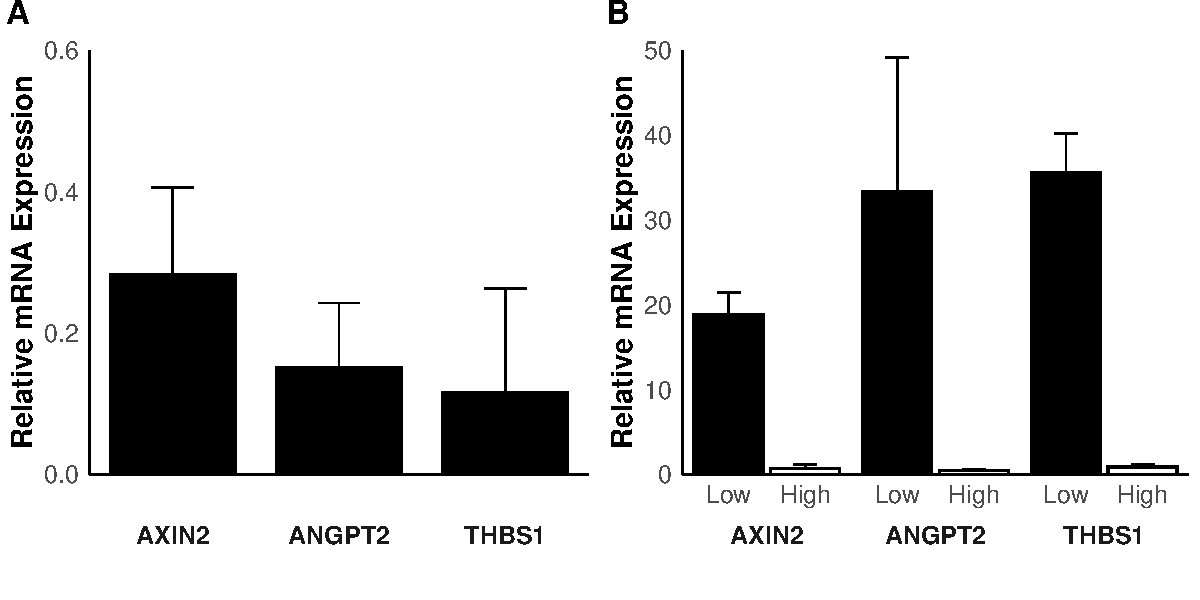
\includegraphics{report_files/figure-latex/plots-1.pdf}
\caption{\label{fig:plots}Cells were treated with DMSO(-) or XAV939(+) and exposed to low or high shear stress. Levels of angiopoeitin-2 , axin-2, and thrombospondin-1 mRNA quantified by qPCR. (\textbf{A}) Data is shown as fold change ± SEM of low shear stress relative to high shear stress. (\textbf{B}) Data is shown as fold change ± SEM of XAV939 relative to DMSO.}
\end{figure}

\hypertarget{discussion}{%
\section{Discussion}\label{discussion}}

\hypertarget{summarise-method-results}{%
\subsection{Summarise Method \& Results}\label{summarise-method-results}}

\hypertarget{inhibitors-axin}{%
\subsection{Inhibitors \& Axin}\label{inhibitors-axin}}

\hypertarget{unreliable-data}{%
\subsection{Unreliable Data}\label{unreliable-data}}

\hypertarget{refine-methods}{%
\subsection{Refine Methods}\label{refine-methods}}

\begin{itemize}
\tightlist
\item
  Methods used in other studies
\end{itemize}

\hypertarget{future-plans}{%
\subsection{Future Plans}\label{future-plans}}

\hypertarget{acknowledgements}{%
\section{Acknowledgements}\label{acknowledgements}}

\begin{flushright}
(669 Words) remove headers !!!
\end{flushright}

\hypertarget{references}{%
\section{References}\label{references}}

\hypertarget{refs}{}
\begin{CSLReferences}{0}{0}
\leavevmode\vadjust pre{\hypertarget{ref-Gelfand2011}{}}%
\CSLLeftMargin{1. }
\CSLRightInline{Gelfand, B. D. {et al.} (2011). {Hemodynamic Activation of ?-Catenin and T-Cell-Specific Transcription Factor Signaling in Vascular Endothelium Regulates Fibronectin Expression}. \emph{Arteriosclerosis, Thrombosis, and Vascular Biology}, 31 (7), pp.1625--1633. {[}Online{]}. Available at: doi:\href{https://doi.org/10.1161/atvbaha.111.227827}{10.1161/atvbaha.111.227827}.}

\leavevmode\vadjust pre{\hypertarget{ref-gordon2006}{}}%
\CSLLeftMargin{2. }
\CSLRightInline{Gordon, M. D. and Nusse, R. (2006). {Wnt Signaling: Multiple Pathways, Multiple Receptors, and Multiple Transcription Factors}. \emph{Journal of Biological Chemistry}, 281 (32), pp.22429--22433. {[}Online{]}. Available at: doi:\href{https://doi.org/10.1074/jbc.r600015200}{10.1074/jbc.r600015200}.}

\leavevmode\vadjust pre{\hypertarget{ref-howe2020}{}}%
\CSLLeftMargin{3. }
\CSLRightInline{Howe, K. L. {et al.} (2020). {Ensembl 2021}. \emph{Nucleic Acids Research}, 49 (D1), pp.D884--D891. {[}Online{]}. Available at: doi:\href{https://doi.org/10.1093/nar/gkaa942}{10.1093/nar/gkaa942}.}

\leavevmode\vadjust pre{\hypertarget{ref-Jho2002}{}}%
\CSLLeftMargin{4. }
\CSLRightInline{Jho, E. {et al.} (2002). {Wnt/?-Catenin/Tcf Signaling Induces the Transcription of Axin2, a Negative Regulator of the Signaling Pathway}. \emph{Molecular and Cellular Biology}, 22 (4), pp.1172--1183. {[}Online{]}. Available at: doi:\href{https://doi.org/10.1128/mcb.22.4.1172-1183.2002}{10.1128/mcb.22.4.1172-1183.2002}.}

\leavevmode\vadjust pre{\hypertarget{ref-Jo2005}{}}%
\CSLLeftMargin{5. }
\CSLRightInline{Jo, W.-S. {et al.} (2005). {Wnt signaling can repress thrombospondin-1 expression in colonic tumorigenesis}. \emph{Cancer Biology \& Therapy}, 4 (12), pp.1361--1366. {[}Online{]}. Available at: doi:\href{https://doi.org/10.4161/cbt.4.12.2201}{10.4161/cbt.4.12.2201}.}

\leavevmode\vadjust pre{\hypertarget{ref-Lustig2002}{}}%
\CSLLeftMargin{6. }
\CSLRightInline{Lustig, B. {et al.} (2002). {Negative Feedback Loop of Wnt Signaling through Upregulation of Conductin/Axin2 in Colorectal and Liver Tumors}. \emph{Molecular and Cellular Biology}, 22 (4), pp.1184--1193. {[}Online{]}. Available at: doi:\href{https://doi.org/10.1128/mcb.22.4.1184-1193.2002}{10.1128/mcb.22.4.1184-1193.2002}.}

\leavevmode\vadjust pre{\hypertarget{ref-Ni2010}{}}%
\CSLLeftMargin{7. }
\CSLRightInline{Ni, C.-W. {et al.} (2010). {Discovery of novel mechanosensitive genes in vivo using mouse carotid artery endothelium exposed to disturbed flow}. \emph{Blood}, 116 (15), pp.e66--e73. {[}Online{]}. Available at: doi:\href{https://doi.org/10.1182/blood-2010-04-278192}{10.1182/blood-2010-04-278192}.}

\leavevmode\vadjust pre{\hypertarget{ref-R}{}}%
\CSLLeftMargin{8. }
\CSLRightInline{R Core Team. (2018). {\emph{R: A language and environment for statistical computing}}. Vienna, Austria: R Foundation for Statistical Computing. {[}Online{]}. Available at: \url{https://www.R-project.org/}.}

\leavevmode\vadjust pre{\hypertarget{ref-Souilhol2020}{}}%
\CSLLeftMargin{9. }
\CSLRightInline{Souilhol, C. {et al.} (2019). {Endothelial responses to shear stress in atherosclerosis: a novel role for developmental genes}. \emph{Nature Reviews Cardiology}, 17 (1), pp.52--63. {[}Online{]}. Available at: doi:\href{https://doi.org/10.1038/s41569-019-0239-5}{10.1038/s41569-019-0239-5}.}

\leavevmode\vadjust pre{\hypertarget{ref-stone2007}{}}%
\CSLLeftMargin{10. }
\CSLRightInline{Stone, P. H. {et al.} (2007). {Regions of low endothelial shear stress are the sites where coronary plaque progresses and vascular remodelling occurs in humans: an in vivo serial study}. \emph{European Heart Journal}, 28 (6), pp.705--710. {[}Online{]}. Available at: doi:\href{https://doi.org/10.1093/eurheartj/ehl575}{10.1093/eurheartj/ehl575}.}

\leavevmode\vadjust pre{\hypertarget{ref-timmins2017}{}}%
\CSLLeftMargin{11. }
\CSLRightInline{Timmins, L. H. {et al.} (2017). {Oscillatory wall shear stress is a dominant flow characteristic affecting lesion progression patterns and plaque vulnerability in patients with coronary artery disease}. \emph{Journal of The Royal Society Interface}, 14 (127), p.20160972. {[}Online{]}. Available at: doi:\href{https://doi.org/10.1098/rsif.2016.0972}{10.1098/rsif.2016.0972}.}

\leavevmode\vadjust pre{\hypertarget{ref-Warboys2019}{}}%
\CSLLeftMargin{12. }
\CSLRightInline{Warboys, C. M., Ghim, M. and Weinberg, P. D. (2019). {Understanding mechanobiology in cultured endothelium: A review of the orbital shaker method}. \emph{Atherosclerosis}, 285, pp.170--177. {[}Online{]}. Available at: doi:\href{https://doi.org/10.1016/j.atherosclerosis.2019.04.210}{10.1016/j.atherosclerosis.2019.04.210}.}

\leavevmode\vadjust pre{\hypertarget{ref-Zhu2017}{}}%
\CSLLeftMargin{13. }
\CSLRightInline{Zhu, J. {et al.} (2017). {Regulation of angiogenic behaviors by oxytocin receptor through Gli1-indcued transcription of HIF-1? in human umbilical vein endothelial cells}. \emph{Biomedicine \& Pharmacotherapy}, 90, pp.928--934. {[}Online{]}. Available at: doi:\href{https://doi.org/10.1016/j.biopha.2017.04.021}{10.1016/j.biopha.2017.04.021}.}

\end{CSLReferences}

\end{document}
